\documentclass[12pt, a4paper]{article}

% !TeX root = ../main.tex
\usepackage{a4wide}

\usepackage[utf8]{inputenc}

%\usepackage[ngerman]{babel}
\usepackage[english]{babel}

\usepackage[T1]{fontenc}
\usepackage{palatino}

\usepackage{graphicx}
\usepackage{caption}
\usepackage{url}
\usepackage{tocloft}
\usepackage{acronym}

\usepackage{mathpazo}
\usepackage{amsmath}
\usepackage{amsfonts}
\usepackage{adjustbox}

%\usepackage{subcaption}

\usepackage{hhline}
\usepackage{amssymb}
\usepackage{floatflt}
\usepackage{setspace}
\usepackage{float}
\usepackage{color}
\usepackage{listings}
\usepackage{array}
\usepackage{scrhack}
\usepackage{xcolor}
\usepackage{wrapfig}
\usepackage{hyperref}
\usepackage{url}
\usepackage{lmodern}
\usepackage{multirow}
\usepackage{subfig}
\usepackage{cleveref}
\usepackage{lipsum}


% !TeX root = ../main.tex
%%%%%%%%%%%%%%%%%%%%%%%%%%%%%%%%%%%%%%%%%%%%%%%%%%%%%%%%%%%%%%%%%%%%%%%%
% Data about you and the Document%
%%%%%%%%%%%%%%%%%%%%%%%%%%%%%%%%%%%%%%%%%%%%%%%%%%%%%%%%%%%%%%%%%%%%%%%%

% % Main Title of Document:
\newcommand{\myMaintitle}{My Main title}

% % Sub Title of DocInput:
\newcommand{\mySubtitle}{My Subtitle}

% % Ihr Name:
\newcommand{\myName}{My Name}

% % Matrikelnummer:
\newcommand{\myMatrikel}{MatNr: XXX}

% % Ihr Geburtsort:
\newcommand{\brith}{City}

% % Ihr Geburtsort:
\newcommand{\place}{City}

% % Ihr Abgabedatum:
\newcommand{\submission}{\today}

% % Ihr Abgabedatum:
\newcommand{\mycourse}{My Course}

% % Name des Betreuers/Erstprüfenden:
\newcommand{\fistSupervisor}{My Supervisor 1}
\newcommand{\secSupervisor}{My Supervisor 2}

% % In welchem Semester befinden Sie sich?
\newcommand{\mySemester}{Semester}

\title{\myMaintitle}

\author{\myName}
% !TeX root = ../main.tex
% % Linespread in main part
%\linespread{1.25}\selectfont

% Line spacing
%\onehalfspacing{}

%Path for Grafiken
\graphicspath{{fig/}}

%Stylerules
\widowpenalty10000 % Vermeidet einzelne Zeilen eines Absatzes zu Beginn einer Seite
\clubpenalty10000 % Vermeidet einzelne Zeilen eines Absatzes am Ende einer Seite
\addtocontents{toc}{\protect\sloppy}
\setcounter{tocdepth}{3}

\renewcommand{\headrulewidth}{.4mm} % header line width


% sloppy no right border override - bigger gabs
\sloppy

% % Set doc properties if 'hyperref' is present.
\hypersetup{pdftitle=\myMaintitle,pdfauthor=\myName,bookmarksopen=true}

% Source for picture captions
\newcommand{\source}[1]{\caption*{Source: {#1}} }

\newcommand{\code}[1]{\texttt{#1}}

\newcommand{\myparagraph}[1]{\paragraph{#1}\mbox{}\\}

\newcommand{\RM}[1]{\MakeUppercase{\romannumeral{} #1{}}}

\newcommand{\HRule}{\rule{\linewidth}{0.5mm}} % Defines a new command for horizontal


\definecolor{dkgreen}{rgb}{0,0.6,0}
\definecolor{gray}{rgb}{0.5,0.5,0.5}
\definecolor{mauve}{rgb}{0.58,0,0.82}

\lstset{ %
  language=Java,                  % the language of the code
  basicstyle=\footnotesize,       % the size of the fonts that are used for the code
  numbers=left,                   % where to put the line-numbers
  numberstyle=\tiny\color{gray},  % the style that is used for the line-numbers
  stepnumber=1,                   % the step between two line-numbers. If it's 1, each line
                                  % will be numbered
  numbersep=5pt,                  % how far the line-numbers are from the code
  backgroundcolor=\color{white},  % choose the background color. You must add \usepackage{color}
  showspaces=false,               % show spaces adding particular underscores
  showstringspaces=false,         % underline spaces within strings
  showtabs=false,                 % show tabs within strings adding particular underscores
  frame=single,                   % adds a frame around the code
  rulecolor=\color{black},        % if not set, the frame-color may be changed on line-breaks within not-black text (e.g. commens (green here))
  tabsize=4,                      % sets default tabsize to 2 spaces
  captionpos=b,                   % sets the caption-position to bottom
  breaklines=true,                % sets automatic line breaking
  breakatwhitespace=false,        % sets if automatic breaks should only happen at whitespace
  title=\lstname,                 % show the filename of files included with \lstinputlisting;
                                  % also try caption instead of title
  keywordstyle=\color{blue},          % keyword style
  commentstyle=\color{dkgreen},       % comment style
  stringstyle=\color{mauve}         % string literal style
}

%%%%%%%%%%%%%%%%%%%%%%%%%%%%%%%%%%%%%%%%%%%%%%%%%%%%%%%%%%%%%%%%%%%%%%%%%%%%%%%%%%%%%%%%%
%Examples
%%%%%%%%%%%%%%%%%%%%%%%%%%%%%%%%%%%%%%%%%%%%%%%%%%%%%%%%%%%%%%%%%%%%%%%%%%%%%%%%%%%%%%%%%
% \pdfmarkupcomment[markup=Squiggly,color=green]{with pdfcomment}{move to the front}.
% \pdfmarkupcomment[markup=StrikeOut,color=red]{stupid}{replace stupid with funny}
% \pdfmarkupcomment[markup=Highlight,color=yellow]{Of course, you can highlight complete sentences.}{Highlight}
% \pdfcomment[icon=Note,color=blue]{insert graphic!}


% \pagestyle{plain}
\pagestyle{fancy}
\fancyhf{}
\fancyhfoffset[L]{1cm} % left extra length
\fancyhfoffset[R]{1cm} % right extra length
\rhead{\thepage}
\lhead{\nouppercase\leftmark}
\cfoot{\fancyplain{}{\thepage} }

\begin{document}
\nocite{*}

\pagenumbering{gobble}
% !TeX root = ../main.tex
%%%%%%%%%%%%%%%%%%%%%%%%%%%%%%%%%%%%%%%%%
% Academic Title Page
% LaTeX Template
% Version 2.0 (17/7/17)
%
% This template was downloaded from:
% http://www.LaTeXTemplates.com
%
% Original author:
% WikiBooks (LaTeX - Title Creation) with modifications by:
% Vel (vel@latextemplates.com)
% hegerdes (hegerdes@uni-osnabrueck.de)
%
% License:
% CC BY-NC-SA 3.0 (http://creativecommons.org/licenses/by-nc-sa/3.0/)
%
% Instructions for using this template:
% This title page is capable of being compiled as is. This is not useful for
% including it in another document. To do this, you have two options:
%
% 1) Copy/paste everything between \begin{document} and \end{document}
% starting at \begin{titlepage} and paste this into another LaTeX file where you
% want your title page.
% OR
% 2) Remove everything outside the \begin{titlepage} and \end{titlepage}, rename
% this file and move it to the same directory as the LaTeX file you wish to add it to.
% Then add \input{./<new filename>.tex} to your LaTeX file where you want your
% title page.
%
%%%%%%%%%%%%%%%%%%%%%%%%%%%%%%%%%%%%%%%%%

%----------------------------------------------------------------------------------------
%	TITLE PAGE
%----------------------------------------------------------------------------------------
%Titelseite
\begin{titlepage}
	\centering
	\thispagestyle{empty}
	\begin{center}
	
\includegraphics[width=0.45\textwidth]{logo.png}
	\end{center}
	\vfill
	\textsc{\Large{\emph{\mycourse}}}\\[0.5cm]
	\HRule\\[0.4cm]
	\vspace{8mm}
	\huge{\textbf{{\fontfamily{ppl}\selectfont
	\myMaintitle}}}\\
	\HRule\\[0.4cm]
	\vspace{9mm}

	\begin{minipage}{0.4\textwidth}
		\begin{flushleft}
			\large
			\textit{Author}\\
			\textsc{\myName}\\ % Your name
			\textsc{\myMatrikel} % Your name
		\end{flushleft}
	\end{minipage}
	~
	\begin{minipage}{0.4\textwidth}
		\begin{flushright}
			\large
			\textit{Supervisor}\\
			\textsc{\fistSupervisor}\\ % Supervisor's name
			\textsc{\secSupervisor} % Supervisor's name
		\end{flushright}
	\end{minipage}

	\vspace{5cm}
	\large{\today}
	\vfill
	\end{titlepage}
	\newpage


\tableofcontents
\newpage
\newcounter{lastroman}
\setcounter{lastroman}{\value{page}}
\pagenumbering{arabic}
\maketitle
\begin{abstract}
    \lipsum[20]
\end{abstract}
\section{Topic1, Content1 and Structure1}
\subsection{Topic}
\lipsum[10]
\subsection{Content}
\lipsum[15]
\begin{figure}[h]
    \centering
    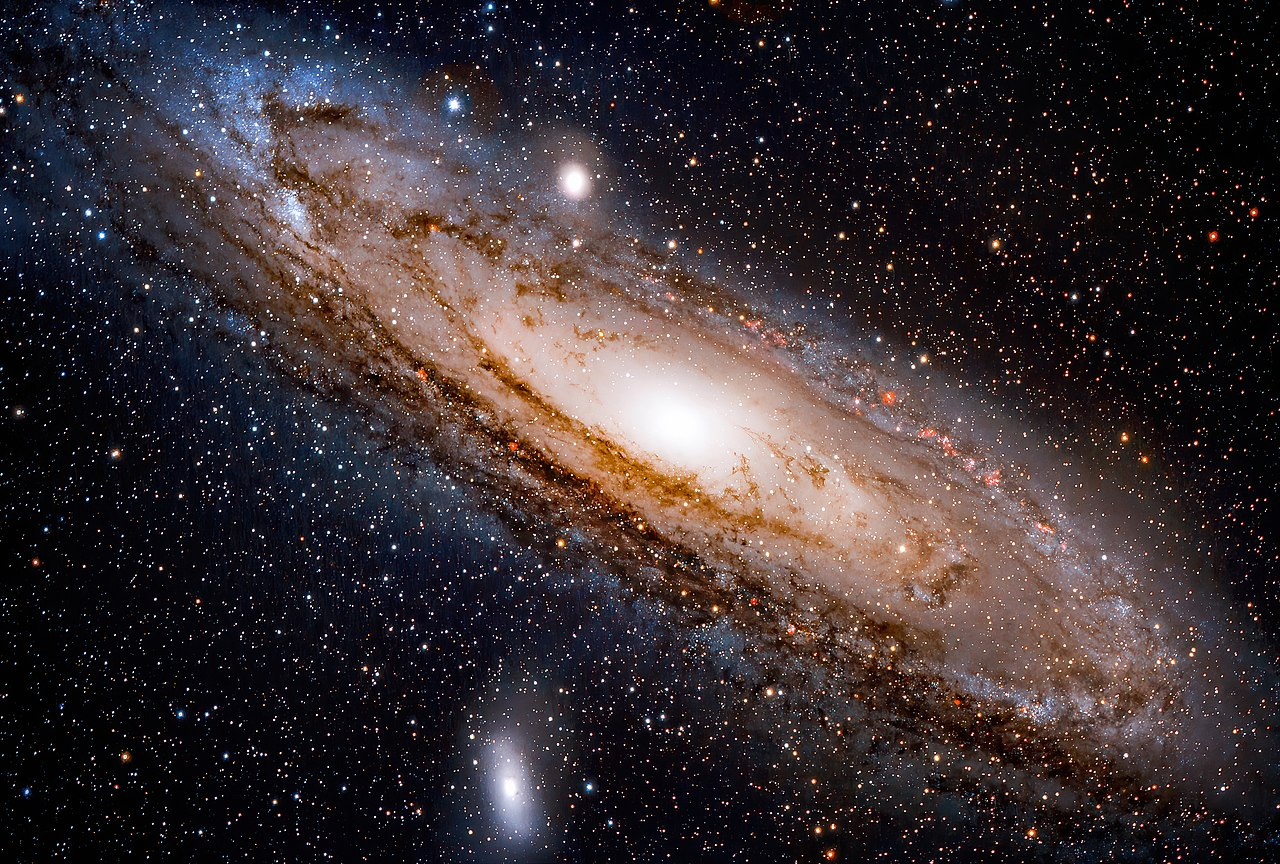
\includegraphics[width=0.65\textwidth]{Andromeda_Galaxy_560mm_FL.jpg}\label{fig::andromeda}
    \caption{Andromeda Galaxy}
\end{figure}
\subsection{Structure}
\lipsum[20]
\section{Topic2, Content2 and Structure2}
\subsection{Topic}
\lipsum[25]
\subsection{Content}
\begin{table}[H]
\centering
\begin{tabular}{@{}llllllll@{}} \toprule
    {\(m\)} & {\(\Re\{\underline{\mathfrak{X}}(m)\}\)} & {\(-\Im\{\underline{\mathfrak{X}}(m)\}\)} & {\(\mathfrak{X}(m)\)} & {\(\frac{\mathfrak{X}(m)}{23}\)} & {\(A_m\)} & {\(\varphi(m)\ /\ ^{\circ}\)} & {\(\varphi_m\ /\ ^{\circ}\)} \\ \midrule
    1  & 16.128 & +8.872 & 16.128 & 1.402 & 1.373 & -146.6 & -137.6 \\
    2  & 3.442  & -2.509 & 3.442  & 0.299 & 0.343 & 133.2  & 152.4  \\
    3  & 1.826  & -0.363 & 1.826  & 0.159 & 0.119 & 168.5  & -161.1 \\
    4  & 0.993  & -0.429 & 0.993  & 0.086 & 0.08  & 25.6   & 90     \\ \midrule
    5  & 1.29   & +0.099 & 1.29   & 0.112 & 0.097 & -175.6 & -114.7 \\
    6  & 0.483  & -0.183 & 0.483  & 0.042 & 0.063 & 22.3   & 122.5  \\
    7  & 0.766  & -0.475 & 0.766  & 0.067 & 0.039 & 141.6  & -122   \\
    8  & 0.624  & +0.365 & 0.624  & 0.054 & 0.04  & -35.7  & 90     \\ \midrule
    9  & 0.641  & -0.466 & 0.641  & 0.056 & 0.045 & 133.3  & -106.3 \\
    10 & 0.45   & +0.421 & 0.45   & 0.039 & 0.034 & -69.4  & 110.9  \\
    11 & 0.598  & -0.597 & 0.598  & 0.052 & 0.025 & 92.3   & -109.3 \\ \bottomrule
\end{tabular}
\caption{Fourier series}\label{tab::fourier}
\end{table}
\subsection{Structure}
\lipsum[35]
\newpage

% Anhang
\renewcommand{\thesubsection}{\Alph{subsection}}
\pagenumbering{Roman}
\setcounter{page}{\value{lastroman}}
\section*{Appendix}
\addcontentsline{toc}{section}{Appendix}

%Abkürzungsverzeichnis
% !TeX root = ../main.tex
\newcommand{\abbr}{Abbreviations}
\subsection{Abbreviations}
%\addcontentsline{toc}{subsection}{Abbreviations}

\begin{acronym}[1234567890]		%[längste Abkürzung]
\setlength{\itemsep}{-\parsep}	% sorgt dafür, dass das Verzeichnis kompakt dargestellt wird.

\acro{OS}[OS]{Operating System}


\end{acronym}
\newpage

%Code
% !TeX root = ../main.tex
\subsection*{Code for you}
\addcontentsline{toc}{subsection}{Code for you}
\begin{lstlisting}[frame=single, caption={DemoCode},label=code::sttf]
    int main(){
        int i;

        // Line comment.
        puts("Hello world!");

        for (i = 0; i < N; i++){
            puts("LaTeX is also great for programmers!");
        }

        return 0;
    }
\end{lstlisting}
\newpage
\listoffigures
\listoftables


%Bibliographie
\addcontentsline{toc}{section}{References}
\bibliographystyle{alpha}
\bibliography{bib/sources}
% !TeX root = ../main.tex
\section*{Declaration of Authorship}

\vspace{5cm}

~\\
I hereby declare that the paper submitted is my own unaided work. I assure that I wrote this paper without using any other means and sources than those specified. As well as the sources used literally or analogously taken from the sources identified as such.

\vspace{3cm}
\begin{flushright}

\rule{8cm}{0.2mm} \\
Signature (\myName)
\end{flushright}

\vspace{2cm}
\place, the \submission{}

\end{document}